\documentclass[12pt, oneside]{article}

\usepackage[letterpaper, scale=0.89, centering]{geometry}
\usepackage{fancyhdr}
\setlength{\parindent}{0em}
\setlength{\parskip}{1em}

\pagestyle{fancy}
\fancyhf{}
\renewcommand{\headrulewidth}{0pt}
\rfoot{\href{https://creativecommons.org/licenses/by-nc-sa/2.0/}{CC BY-NC-SA 2.0} Version \today~(\thepage)}

\usepackage{amssymb,amsmath,pifont,amsfonts,comment,enumerate,enumitem}
\usepackage{currfile,xstring,hyperref,tabularx,graphicx,wasysym}
\usepackage[labelformat=empty]{caption}
\usepackage[dvipsnames,table]{xcolor}
\usepackage{multicol,multirow,array,listings,tabularx,lastpage,textcomp,booktabs}

\lstnewenvironment{algorithm}[1][] {   
    \lstset{ mathescape=true,
        frame=tB,
        numbers=left, 
        numberstyle=\tiny,
        basicstyle=\rmfamily\scriptsize, 
        keywordstyle=\color{black}\bfseries,
        keywords={,procedure, div, for, to, input, output, return, datatype, function, in, if, else, foreach, while, begin, end, }
        numbers=left,
        xleftmargin=.04\textwidth,
        #1
    }
}
{}
\lstnewenvironment{java}[1][]
{   
    \lstset{
        language=java,
        mathescape=true,
        frame=tB,
        numbers=left, 
        numberstyle=\tiny,
        basicstyle=\ttfamily\scriptsize, 
        keywordstyle=\color{black}\bfseries,
        keywords={, int, double, for, return, if, else, while, }
        numbers=left,
        xleftmargin=.04\textwidth,
        #1
    }
}
{}

\newcommand\abs[1]{\lvert~#1~\rvert}
\newcommand{\st}{\mid}

\newcommand{\A}[0]{\texttt{A}}
\newcommand{\C}[0]{\texttt{C}}
\newcommand{\G}[0]{\texttt{G}}
\newcommand{\U}[0]{\texttt{U}}

\newcommand{\cmark}{\ding{51}}
\newcommand{\xmark}{\ding{55}}

 
\begin{document}
\begin{flushright}
    \StrBefore{\currfilename}{.}
\end{flushright} \section*{Week4 monday}


Recap so far: In DFA, the only memory available is in the states. Automata can only
``remember'' finitely far in the past and finitely much information, because
they can have only finitely many states. If a computation path of a DFA visits 
the same state more than once, the machine can't tell the difference between 
the first time and future times it visits this state. Thus, if 
a DFA accepts one long string, then it must accept (infinitely) many 
similar strings.

{\bf Definition}  A positive integer $p$ is a {\bf pumping length} of a language $L$ over $\Sigma$ means
that, for each string $s  \in  \Sigma^*$, if  $|s| \geq p$ and $s \in L$, then there are strings $x,y,z$
such that 
\[
s = xyz
\]
and  
\[
|y| > 0,  \qquad \qquad 
\text{ for each $i \geq 0$, $xy^i z \in L$}, \qquad \text{and}
\qquad  \qquad
|xy| \leq p.
\]

{\bf Negation}: A positive integer  $p$  is {\bf not a pumping length} of a language  $L$ over  $\Sigma$  iff
\[
\exists s \left(~  |s| \geq  p \wedge s \in L \wedge \forall x \forall y \forall z  \left( ~\left( s = xyz \wedge 
|y| > 0 \wedge |xy| \leq p~ \right) \to \exists i  (  i \geq 0  \wedge xy^iz  \notin L ) \right) ~\right) 
\]
{\it Informally: }


Restating {\bf Pumping Lemma}: If $L$ is a regular language, then it  has
a pumping length.


{\bf Contrapositive}: If $L$ has no pumping length, then  it is nonregular.

\vfill

{\Large The Pumping Lemma {\it cannot} be used to prove that a language {\it is} regular.} 

{\Large The Pumping Lemma {\bf can} be used to prove that a language {\it is not} regular.}

{\it Extra practice}: Exercise 1.49 in the book.


\vfill

{\bf Proof strategy}: To prove that a language $L$ is {\bf not} regular, 
\begin{itemize}
    \item Consider an arbitrary positive integer $p$
    \item Prove that $p$ is not a pumping length for $L$
    \item Conclude that $L$ does not have {\it any} pumping length, and therefore it is not regular.
\end{itemize}

\newpage
{\bf Example}: $\Sigma  =  \{0,1\}$, $L = \{ 0^n 1^n \mid n  \geq 0\}$.

Fix $p$ an arbitrary positive integer. List strings that are in $L$ and have length  greater than or equal  to $p$:

\vspace{20pt}

Pick $s = $


Suppose $s = xyz$ with  $|xy|  \leq  p$ and $|y| > 0$.
\begin{center}
\begin{tabular}{|c|}
\hline
 \\
\hspace{4in} \\
\hline
\end{tabular}
\end{center}

Then when $i = \hspace{1in}$, $xy^i z  = \hspace{1in}$

\newpage

{\bf Example}: $\Sigma  =  \{0,1\}$, $L = \{w w^{\mathcal{R}} \mid w \in \{0,1\}^*\}$.

Fix $p$ an arbitrary positive integer. List strings that are in $L$ and have length  greater than or equal  to $p$:

\vspace{10pt}

Pick $s = $

Suppose $s = xyz$ with  $|xy|  \leq  p$ and $|y| > 0$.
\begin{center}
\begin{tabular}{|c|}
\hline
 \\
\hspace{4in} \\
\hline
\end{tabular}
\end{center}
Then when $i = \hspace{1in}$, $xy^i z  = \hspace{1in}$


\vspace{30pt} 

{\bf Example}: $\Sigma  =  \{0,1\}$, $L = \{0^j1^k  \mid j \geq k  \geq 0\}$.

Fix $p$ an arbitrary positive integer. List strings that are in $L$ and have length  greater than or equal  to $p$:

\vspace{10pt}

Pick $s = $


Suppose $s = xyz$ with  $|xy|  \leq  p$ and $|y| > 0$.
\begin{center}
\begin{tabular}{|c|}
\hline
 \\
\hspace{4in} \\
\hline
\end{tabular}
\end{center}
Then when $i = \hspace{1in}$, $xy^i z  = \hspace{1in}$



\vspace{30pt} 

{\bf Example}: $\Sigma  =  \{0,1\}$, $L = \{0^n1^m0^n  \mid m,n  \geq 0\}$.

Fix $p$ an arbitrary positive integer. List strings that are in $L$ and have length  greater than or equal  to $p$:

\vspace{10pt}

Pick $s = $


Suppose $s = xyz$ with  $|xy|  \leq  p$ and $|y| > 0$.
\begin{center}
\begin{tabular}{|c|}
\hline
 \\
\hspace{4in} \\
\hline
\end{tabular}
\end{center}
Then when $i = \hspace{1in}$, $xy^i z  = \hspace{1in}$
 \vfill
\section*{Week4 wednesday}



\begin{center}
    \begin{tabular}{c|c| c| c}
    Language & $s \in L$ & $s \notin L$ & Is the language regular or nonregular?  \\
    \hline
     & \hspace{1in} & \hspace{1in}  &  \\
    $\{a^nb^n \mid 0  \leq n  \leq 5 \}$ & & & \\
     & & & \\
    $\{b^n a^n \mid  n  \geq 2\}$  & & & \\
     & & & \\
    $\{a^m b^n \mid  0 \leq m\leq n\}$  & & & \\
     & & & \\
    $\{a^m b^n \mid  m \geq n+3,  n \geq 0\}$  & & & \\
     & & & \\
    $\{b^m a^n \mid  m \geq 1, n \geq  3\}$  & & & \\
     & & & \\
    $\{ w  \in \{a,b\}^* \mid w = w^\mathcal{R} \}$ & & & \\
     & & & \\ 
    $\{ ww^\mathcal{R} \mid w\in \{a,b\}^* \}$ & & & \\
     & & & \\ 
    \end{tabular}
\end{center}
    
\newpage
Regular sets are not the end of the story
\begin{itemize}
    \item Many nice / simple / important sets are not regular
    \item Limitation of the finite-state automaton model: Can't "count", Can only remember finitely far into the past,
    Can't backtrack, Must make decisions in "real-time"
    \item We know actual computers are more powerful than this model...
\end{itemize}

The {\bf next} model of computation. Idea: allow some memory of unbounded size. How? 
\begin{itemize}
    \item To generalize regular expressions: {\bf context-free grammars}\\
    \item To generalize NFA: {\bf Pushdown automata}, which is like an NFA with access to a stack: 
    Number of states is fixed, number of entries in stack is unbounded. At each step
    (1) Transition to new state based on current state, letter read, and top letter of stack, then
    (2) (Possibly) push or pop a letter to (or from) top of stack. Accept a string iff
    there is some sequence of states and some sequence of stack contents 
    which helps the PDA processes the entire input string and ends in an accepting state.
\end{itemize}

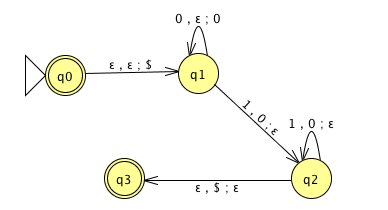
\includegraphics[width=4in]{resources/machines/Lect9PDA.png}
    
Trace the computation of this PDA on the input string $01$.

\vspace{80pt}  
    
Trace the computation of this PDA on the input string $011$.

\vspace{80pt}
 \vfill
\section*{Week4 friday}


{\bf Definition} A {\bf pushdown automaton} (PDA) is  specified by a  $6$-tuple $(Q, \Sigma, \Gamma, \delta, q_0, F)$
where $Q$ is the finite set of states, $\Sigma$ is the input alphabet,  $\Gamma$ is the stack alphabet,
\[
    \delta: Q \times \Sigma_\varepsilon  \times  \Gamma_\varepsilon \to \mathcal{P}( Q \times \Gamma_\varepsilon)
\]
is the transition function,  $q_0 \in Q$ is the start state, $F \subseteq  Q$ is the set of accept states.
    
\begin{multicols}{2}
    {\it Formal definition}
    
    \vspace{90pt}
    Draw the state diagram of a PDA with $\Sigma = \Gamma$.
    
    \columnbreak 
    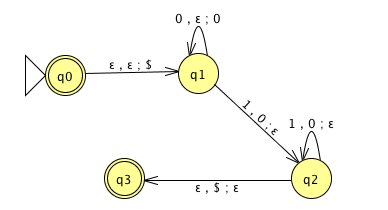
\includegraphics[height=100pt]{resources/machines/Lect9PDA.png}
    
    
    Draw the state diagram of a PDA with $\Sigma \cap \Gamma = \emptyset$.
    
\end{multicols}
    
\vspace{60pt}
    
A PDA recognizing the set $\{ \hspace{1.5 in} \}$ can be informally described as:
\begin{quote}
    Read symbols from the input. As each 0 is read, push it onto the stack. As soon as 1s are seen, pop a 0 off the stack for each 1 read. If the stack becomes empty and there is exactly one 1 left to read, read that 1 and accept the input. If the stack becomes empty and there are either zero or more than one 1s left to read, or if the 1s are finished while the stack still contains 0s, or if any 0s appear in the input following 1s, reject the input.
\end{quote}
    
    State diagram for this  PDA:

    
\vfill
\newpage
Consider the state diagram of a PDA with input alphabet 
$\Sigma$ and stack alphabet $\Gamma$.

\begin{center}
\begin{tabular}{|c|c|}
\hline
Label & means \\
\hline
$a, b ; c$ when $a \in \Sigma$, $b\in \Gamma$, $c \in \Gamma$ 
& \hspace{3in} \\
& \\
&\\
\hline
$a, \varepsilon ; c$ when $a \in \Sigma$, $c \in \Gamma$ 
& \hspace{3in} \\
& \\
&\\
\hline
$a, b ; \varepsilon$ when $a \in \Sigma$, $b\in \Gamma$
& \hspace{3in} \\
& \\
&\\
\hline
$a, \varepsilon ; \varepsilon$ when $a \in \Sigma$
& \hspace{3in} \\
& \\
&\\
\hline
\end{tabular}
\end{center}


How does the meaning change if $a$ is replaced by $\varepsilon$?

{\it Note: alternate notation is to replace $;$ with $\to$}


For the PDA state diagrams below, $\Sigma = \{0,1\}$.


\begin{center}
\begin{tabular}{c c}
Mathematical description of language & State diagram of PDA recognizing language\\
\hline
& 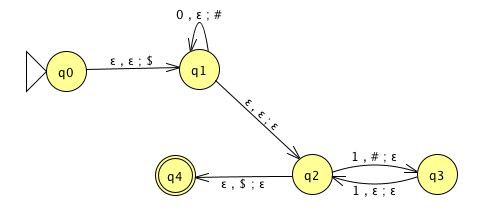
\includegraphics[width=3.5in]{resources/machines/Lect10PDA1.png}\\
\hline
& 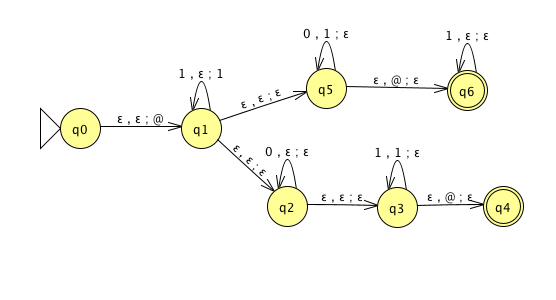
\includegraphics[width=3.5in]{resources/machines/Lect10PDA2.png}\\
\hline
& \\
$\{ 0^i 1^j 0^k \mid i,j,k \geq 0 \}$ & \\
\end{tabular}
\end{center}
 \vfill
\section*{Week3 friday}



{\bf Theorem}: For an alphabet $\Sigma$, For each language $L$ over $\Sigma$, 
\begin{center}
$L$ is recognized by some DFA \\
iff\\
$L$ is recognized by some NFA\\
iff\\
$L$ is described by some regular expression
\end{center}
If (any, hence all) these conditions apply, $L$ is called {\bf regular}.



{\bf Prove or Disprove}: There is some alphabet $\Sigma$ for which there is 
some language recognized by an NFA but not by any DFA.

\vspace{30pt}

{\bf Prove or Disprove}: There is some alphabet $\Sigma$ for which there is 
some finite language not described by any regular expression over $\Sigma$.

\vspace{30pt}


{\bf Prove or Disprove}: If a language is recognized by an NFA 
then the complement of this language is not recognized by any DFA.

\vspace{30pt}


\newpage
\begin{center}
\begin{tabular}{c|c}
Set & Cardinality \\
\hline
& \\
$\{0,1\}$ & \\
& \\
$\{0,1\}^*$ & \\
& \\
$\mathcal{P}( \{0,1\})$ & \\
& \\
The set of all languages over $\{0,1\}$ & \\
& \\
The set of all regular expressions over $\{0,1\}$ & \\
& \\
The set of all regular languages over $\{0,1\}$ & \\
& \\
\end{tabular}
\end{center}



\vfill

\newpage

{\bf Pumping Lemma} (Sipser Theorem 1.70): If $A$ is a regular language, then there
is a number $p$ (a {\it pumping length}) where, if $s$ is any string in $A$ of length at least $p$, 
then $s$ may be divided into three pieces, $s = xyz$ such that
\vspace{-10pt}
\begin{itemize}
\item $|y| > 0$
\item for each $i \geq 0$, $xy^i z \in A$
\item $|xy| \leq p$.
\end{itemize}


{\bf True or False}: A pumping length for $A = \{ 0,1 \}^*$ is $p = 5$.

\vspace{100pt}

{\bf True or False}: A pumping length for $A = \{1, 01, 001, 0001, 00001 \}$ is $p = 4$.

\vspace{100pt}

{\bf True or False}: A pumping length for $A = \{0^j 1 \mid  j \geq 0 \}$ is $p = 3$.


\vspace{100pt}

{\bf True or False}: For any language $A$, if $p$  is a  pumping length for $A$ and $p' > p$,  then 
$p'$ is also a pumping length for $A$.
 \vfill
\end{document}